% Conceptual regime map: action correctness x legitimacy. Compile: pdflatex fig_regimemap.tex
\documentclass[border=6pt]{standalone}
\usepackage{amsmath,amssymb}
\usepackage{tikz}
\usetikzlibrary{arrows.meta,positioning,fit}
\begin{document}
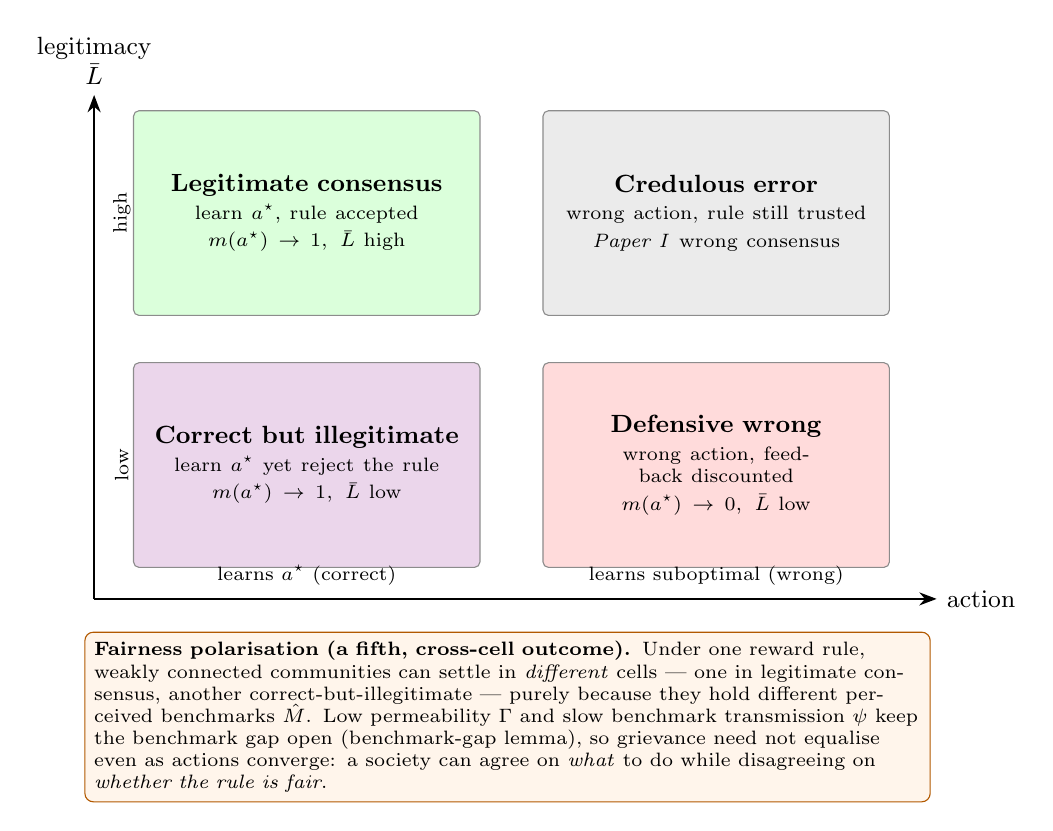
\begin{tikzpicture}[font=\small,>={Stealth[length=2.2mm]},
  cell/.style={minimum width=44mm,minimum height=26mm,align=center,
               draw=black!45,rounded corners=2pt,text width=40mm}]
% cells (x: correct left / wrong right ; y: high L top / low L bottom)
\node[cell,fill=green!14]  (LC) at (0,0)   {\textbf{Legitimate consensus}\\[2pt]\scriptsize learn $a^\star$, rule accepted\\[-1pt]\scriptsize $m(a^\star)\!\to\!1,\ \bar L$ high};
\node[cell,fill=black!8]   (WC) at (5.2,0) {\textbf{Credulous error}\\[2pt]\scriptsize wrong action, rule still trusted\\[-1pt]\scriptsize \emph{Paper~I} wrong consensus};
\node[cell,fill=violet!16] (CI) at (0,-3.2){\textbf{Correct but illegitimate}\\[2pt]\scriptsize learn $a^\star$ yet reject the rule\\[-1pt]\scriptsize $m(a^\star)\!\to\!1,\ \bar L$ low};
\node[cell,fill=red!14]    (DW) at (5.2,-3.2){\textbf{Defensive wrong}\\[2pt]\scriptsize wrong action, feedback discounted\\[-1pt]\scriptsize $m(a^\star)\!\to\!0,\ \bar L$ low};
% axes
\draw[->,thick] (-2.7,-4.9) -- (-2.7,1.5) node[above,align=center]{legitimacy\\$\bar L$};
\node[rotate=90,font=\scriptsize] at (-2.35,0.0){high};
\node[rotate=90,font=\scriptsize] at (-2.35,-3.2){low};
\draw[->,thick] (-2.7,-4.9) -- (8.0,-4.9) node[right,align=center]{action};
\node[font=\scriptsize] at (0,-4.6){learns $a^\star$ (correct)};
\node[font=\scriptsize] at (5.2,-4.6){learns suboptimal (wrong)};
% fairness polarisation = communities occupy different cells (prose, no arrows)
\node[draw=orange!70!black,rounded corners=3pt,fill=orange!8,text width=105mm,align=left,
      font=\scriptsize] (FP) at (2.55,-6.4)
   {\textbf{Fairness polarisation (a fifth, cross-cell outcome).} Under one reward
    rule, weakly connected communities can settle in \emph{different} cells --- one
    in legitimate consensus, another correct-but-illegitimate --- purely because
    they hold different perceived benchmarks $\hat M$. Low permeability $\Gamma$
    and slow benchmark transmission $\psi$ keep the benchmark gap open
    (benchmark-gap lemma), so grievance need not equalise even as actions
    converge: a society can agree on \emph{what} to do while disagreeing on
    \emph{whether the rule is fair}.};
\end{tikzpicture}
\end{document}
